% !TEX root =  ../main_manuscript.tex 
\section{Introduction}
Patients with low- and very low-risk screening-detected localized prostate cancer are usually advised active surveillance (AS) instead of immediate radical treatment~\citep{briganti2018active}. In AS, cancer progression is routinely monitored via prostate-specific antigen (PSA), digital rectal examination, and repeat biopsies. Among these, the strongest indicator of cancer-related outcomes is the biopsy Gleason grade~\citep{epsteinGG2014}. When the Gleason grade increases from grade~1 (Gleason 3+3) to 2 (Gleason 3+4) or higher, called \textit{reclassification}, patients are commonly advised curative treatment~\citep{bul2013active}.

\begin{figure}
\centerline{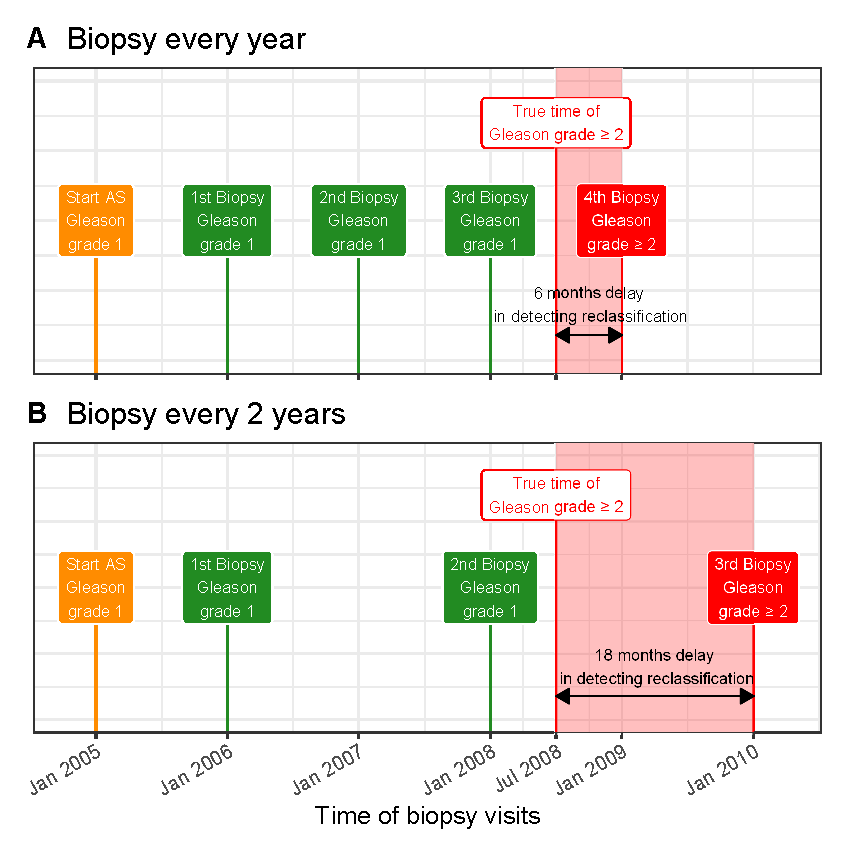
\includegraphics[width=\columnwidth]{images/delay_explanation.eps}}
\caption{\textbf{Trade-off between the number of biopsies and time delay in detecting reclassification (Increase in Gleason grade from 1 to 2 or higher):} The true time of reclassification for the patient in this figure is July 2008. When biopsies are scheduled annually (\textbf{Panel~A}), reclassification is detected in January 2009 with a time delay of six months, and a total of four biopsies are scheduled. When biopsies are scheduled biennially (\textbf{Panel~B}) reclassification is detected in January 2010 with a time delay of 18 months, and a total of three biopsies are scheduled. Since biopsies are conducted periodically, the time of reclassification is observed as an interval. For example, between Jan~2008--Jan~2009 in \textbf{Panel~A} and between Jan~2008--Jan~2010 in \textbf{Panel~B}.}
\label{fig:delay_explanation}
\end{figure}

Biopsies are conducted periodically. Consequently, reclassification is always detected with a time delay (Figure~\ref{fig:delay_explanation}). For detecting reclassification timely, many AS programs schedule fixed and frequent biopsies (e.g.,~annually) for all patients~\citep{nieboer2018active,loeb2014heterogeneity}. However, this also leads to many unnecessary biopsies in slow/non-progressing patients. Biopsies are invasive, painful and prone to medical complications. Thus, biopsy burden and patient non-compliance to frequent biopsies~\citep{bokhorst2015compliance} has raised concerns regarding the optimal biopsy schedule~\citep{inoue2018comparative, bratt2013study}. To this end, infrequent schedules such as biennial biopsies have been proposed as an alternative~\citep{inoue2018comparative,de2017estimating}. Although, biennial biopsies may still lead to five unnecessary biopsies over ten years (current study period of large AS programs) for slow/non-progressing patients. A promising alternative to fixed and frequent biopsies is personalized biopsy schedules based on the patient-specific risk of reclassification (Figure~\ref{fig:riskBasedExample}).

\begin{figure}
\centerline{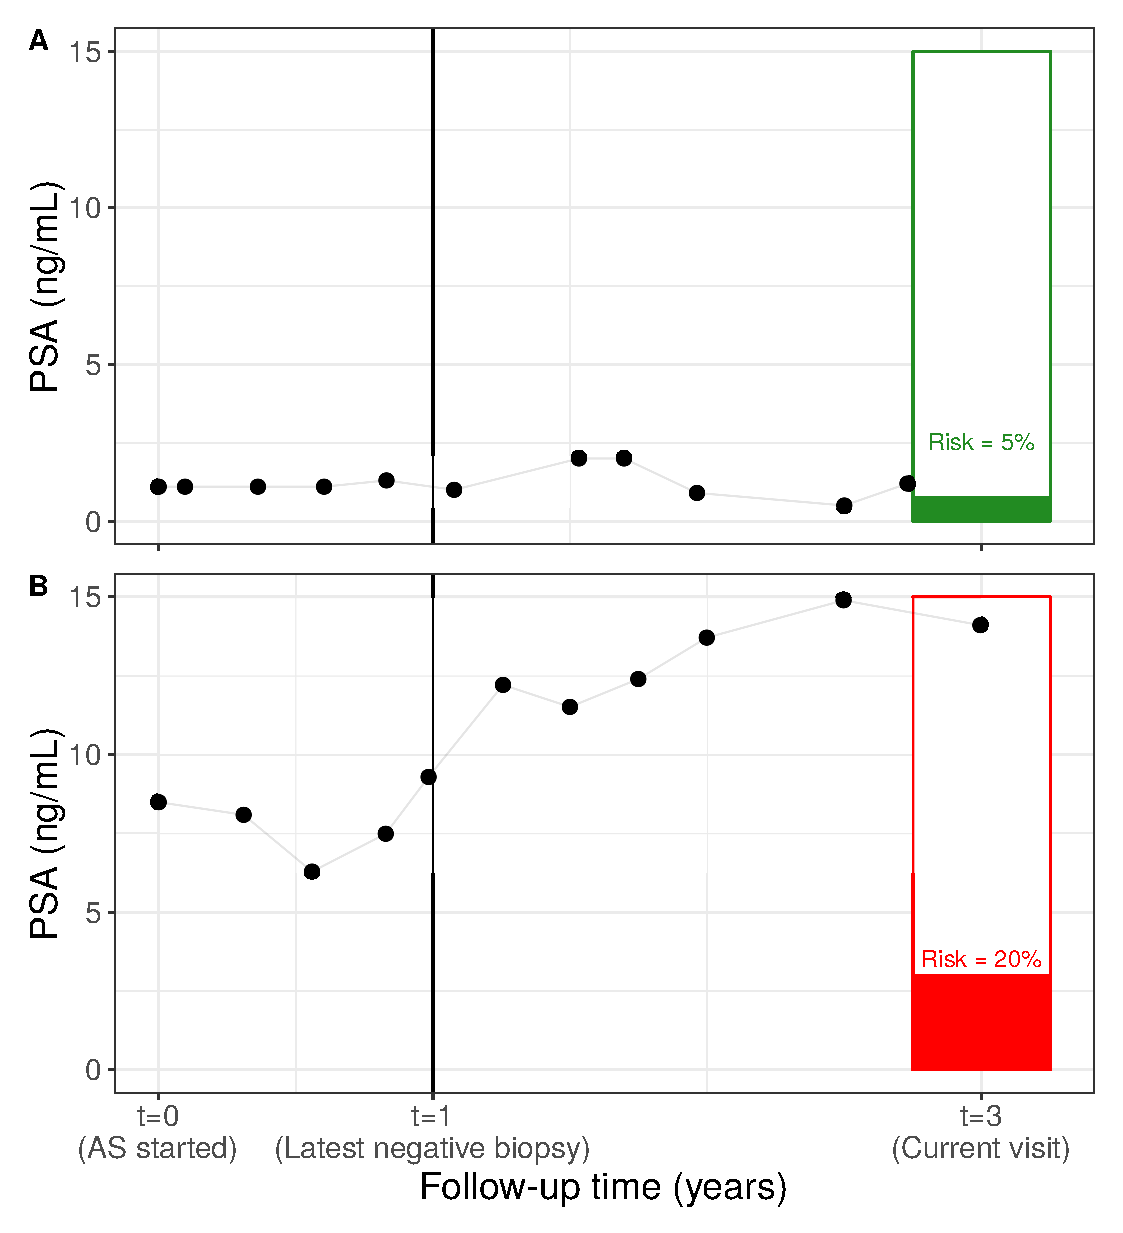
\includegraphics[width=\columnwidth]{images/riskBasedExample.eps}}
\caption{\textbf{Motivation for personalized risk-based decisions of biopsy}: Patient~A (\textbf{Panel~A}) and B (\textbf{Panel~B}) had their latest biopsy at year one of follow-up (green vertical line). Patient~A's prostate-specific antigen (PSA) profile remained stable until his current visit at year three, whereas patient~B's profile has shown a rise. Consequently, patient~B's estimated cumulative risk of reclassification at the current visit (year three) is higher than that of patient~A. This makes patient~B a more suitable candidate for biopsy than Patient~A. Risk estimates in this figure are only illustrative.}
\label{fig:riskBasedExample}
\end{figure}

The first challenge in developing personalized biopsy schedules is consolidating accumulated patient data (e.g., PSA, previous biopsy results) into risk estimates for reclassification. Existing calculators for risk of reclassification~\citep{partin1993use,makarov2007updated} use only the latest PSA measurement of a patient. In contrast, we intend to utilize all repeated measurements of PSA, previous biopsy results, and baseline characteristics of a patient. To this end, a suitable model is the joint model for time-to-event and longitudinal data~\citep{tomer2019, coley2017prediction,rizopoulos2012joint}. A joint model predicts risk of reclassification in a personalized manner. A subsequent challenge however, is translating risks into clinical decisions. For example, a 10\% risk of reclassification can be perceived high/low depending upon the patient age. Patients may also weigh risks of reclassification with the potential \textit{consequences} of another biopsy. Two relevant \textit{consequences} of biopsies (Figure~\ref{fig:delay_explanation}) are the timing and total number of biopsies (burden), and the time delay in detecting reclassification (smaller is beneficial). The relative importance of these \textit{consequences} can vary between the patients, and also over the follow-up period for the same patient.

The goal of this work was to assist patients and doctors in making better decisions of biopsies than fixed and frequent biopsies. For this purpose, we developed a web-application that gives patients their current and future risk of reclassification. It also suggests them risk-based personalized schedules of biopsies. For each biopsy schedule, be it fixed or personalized, the web-application provides expected \textit{consequences} of following it. Thus, patients can compare schedules before making a decision. The web-application uses a prediction joint model fitted to the world's largest AS dataset, PRIAS~\citep{bul2013active}. We externally validated this model in five largest AS cohorts of the GAP3 database \citep{gap3_2018}. Thus, the web-application can be used by a large number of patients worldwide.